%\documentclass[11pt]{amsproc}
%\documentclass[11pt]{article}
\documentclass[11pt]{article}
%\usepackage{setspace}
%\usepackage{fancyhdr}
\usepackage{fullpage}
\usepackage{graphicx}
\usepackage{amssymb}
%\usepackage{accents}
\usepackage{amsfonts}
\usepackage{amsthm}
\usepackage{amsmath}
\usepackage{eucal}
\usepackage{xypic}
\usepackage{pdfsync}
\usepackage{hyperref}
\usepackage{enumerate}



%%\setrightmargin{1in}
%\setallmargins{1in}

% Titlerule is a FAT ruler
\newcommand{\titlerule}{\rule{\linewidth}{1.5mm}}
% For comments in the draft - work in progress
\newcommand{\betainsert}[2]{\fbox{#1}\marginnote{\textsf{#2}}}

% Notes in the margin are nicer this way. HaHa
\newcommand{\marginnote}[1]{\marginpar{\scriptsize\raggedright #1}}



\def\bd{\partial}
\def\ra{\rightarrow}
\def\lra{\longrightarrow}
\def\Z{{\mathbb Z}}
\def\N{{\mathbb N}}
\def\R{{\mathbb R}}
\def\Q{{\mathbb Q}}
\def\C{{\mathbb C}}
\def\P{{\mathbb P}}
\def\K{{\mathbb K}}
\def\w{\mathcal{W}(E)}
\def\A{\mathcal{A}}
\def\B{\mathcal{B}}
\def\M{\mathcal{M}}
\def\N{\mathcal{N}}
\def\p{\partial}

\newcommand*{\longhookrightarrow}{\ensuremath{\lhook\joinrel\relbar\joinrel\rightarrow}}

\newtheorem{lem}{Lemma}
\newtheorem{prop}{Proposition}
\newtheorem{thm}{Theorem}
\newtheorem{cor}{Corollary}
\newtheorem{conj}{Conjecture}
\newtheorem{defn}{Definition}
\newtheorem{claim}{Claim}
\newtheorem{ques}{Question}
\newtheorem{rem}{Remark}

\theoremstyle{remark}
\newtheorem*{prob}{Problem}
\newtheorem{ex}{Example}
\def\T{\mathbb{T}}

\begin{document}
\begin{center}
    \begin{Large} {\bf Math 540 Homework 5}\\
    \end{Large}
    Haosen Wu  / Thur, Spet. 27, 2018
\end{center}
%\vspace{10mm}


\subsection*{1 }
\indent a. We identify $\C=\R^2$, as corollary of Homework 4.1 we know that $\pi_1(\C-\{-2,-1,-0,1\};2)=\Z*\Z*\Z*\Z$ and $\pi_1(\C-\{0,1\};4)=\Z*\Z$.\\

b. By Figure $1$ and we identify the action of $f(z)$ as rotate $Arg(z)$ and stretch $2$ times. We also recognize that generators of fundamental group as loop elements.  We have then, correspond the pushout $f_*$ sending $[x_1x_2x_3x_4],[x_2x_3x_4],[x_3x_4],[x_4] \in \pi_1(\C-\{-2,-1,-0,1\};2)=\Z*\Z*\Z*\Z$ to $[y_1y_2y_1y_2 ],[y_1y_2y_1y_2],[{y_1}^2 y_2],[y_2] \in \pi_1(\C-\{-0,1\};2)=\Z*\Z$.(See Figure $1$, elements are represented by ellipses in order.)

Calculation then shows: $[x_1],[x_2],[x_3],[x_4] \in \pi_1(\C-\{-2,-1,-0,1\};2)=\Z*\Z*\Z*\Z$ to $[1],[y_1y_2{y_1}^{-1}],[{y_1}^2],[y_2] \in \pi_1(\C-\{-0,1\};2)=\Z*\Z$. As all elements in loop space are from generators, we acquire $f_*$ by juxtaposing each $f_*([x_i])$.

A  diagram is below (Figure 1).
    \begin{figure}[h!]
    \centering
    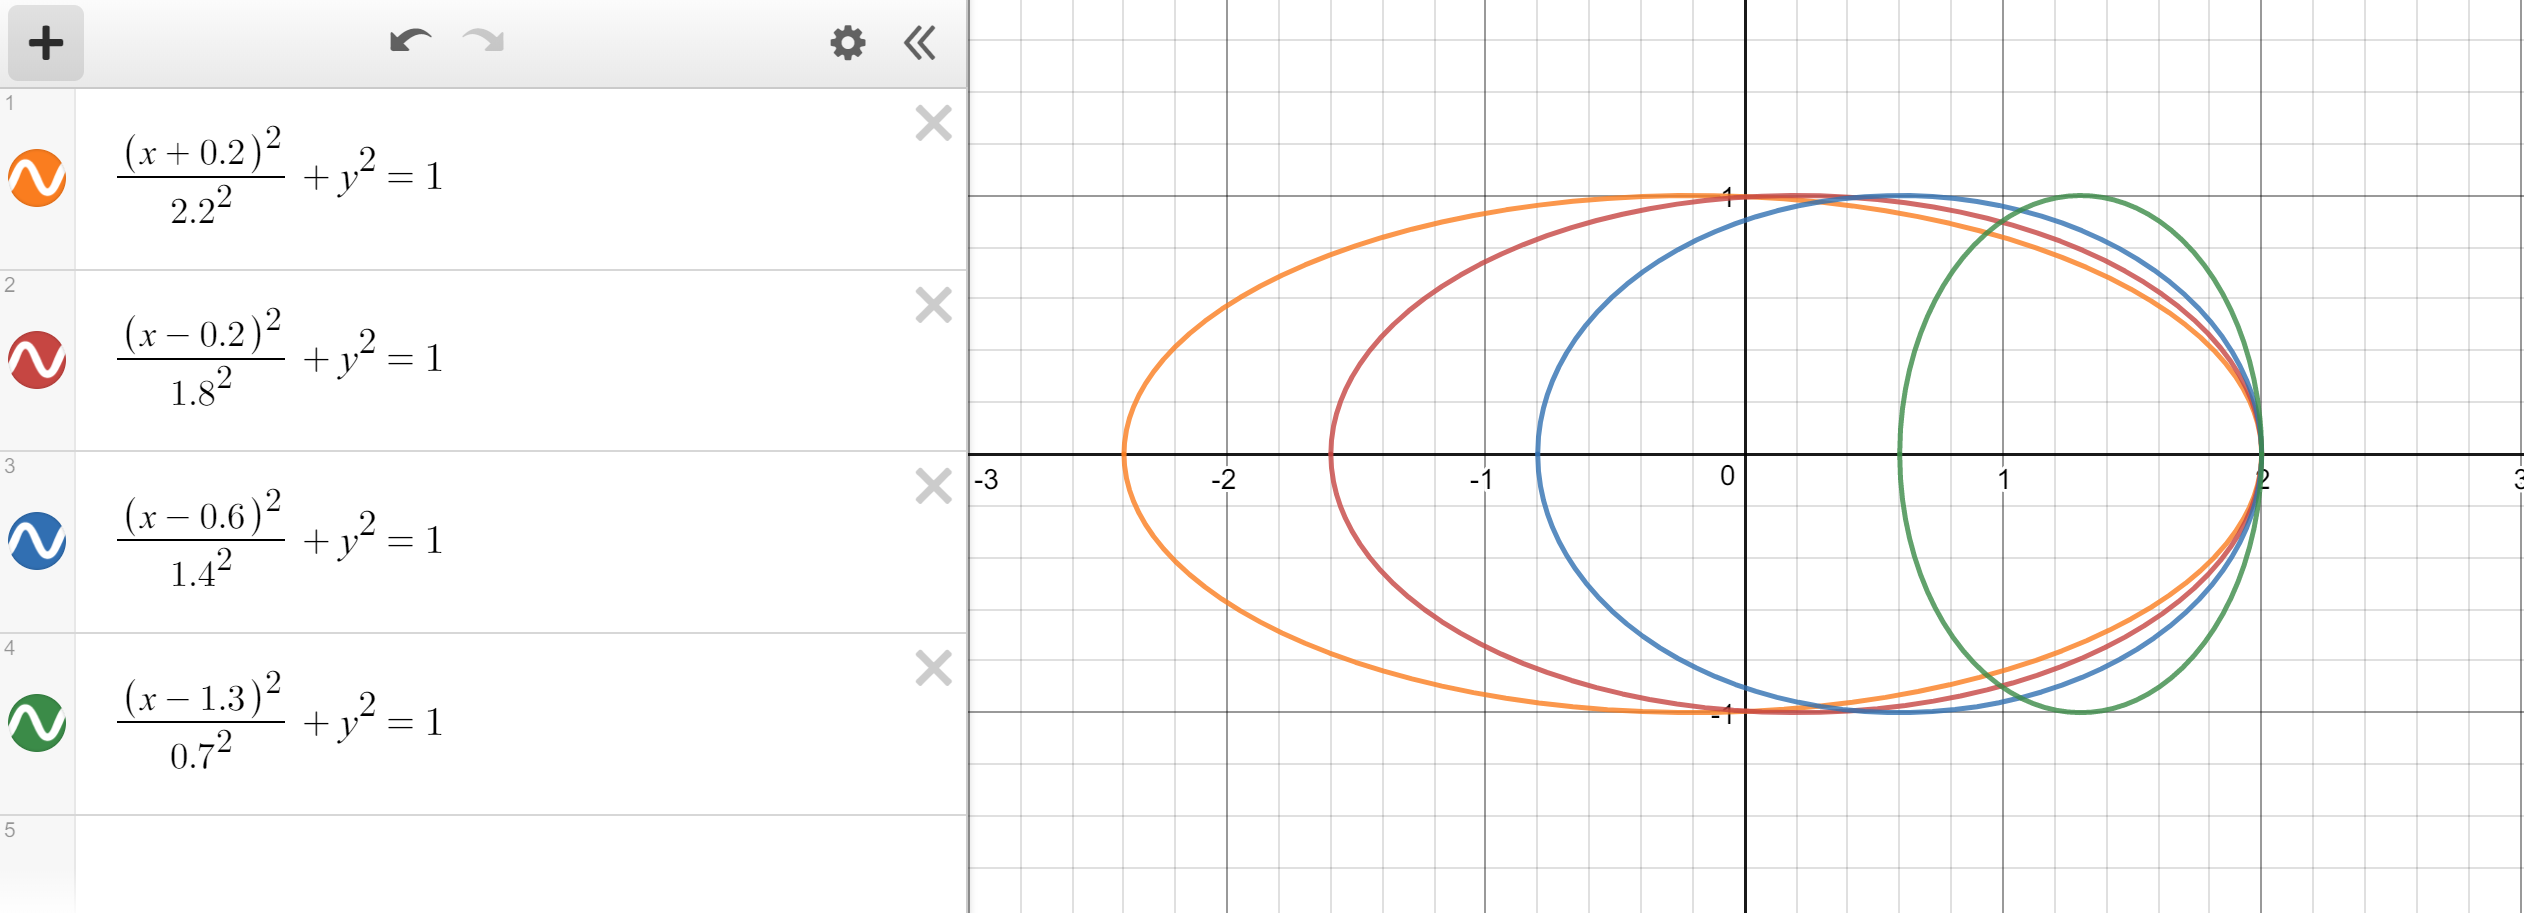
\includegraphics[scale=0.33]{5she1}
    \caption{1-1}
    \end{figure}
    \begin{figure}[h!]
    \centering
    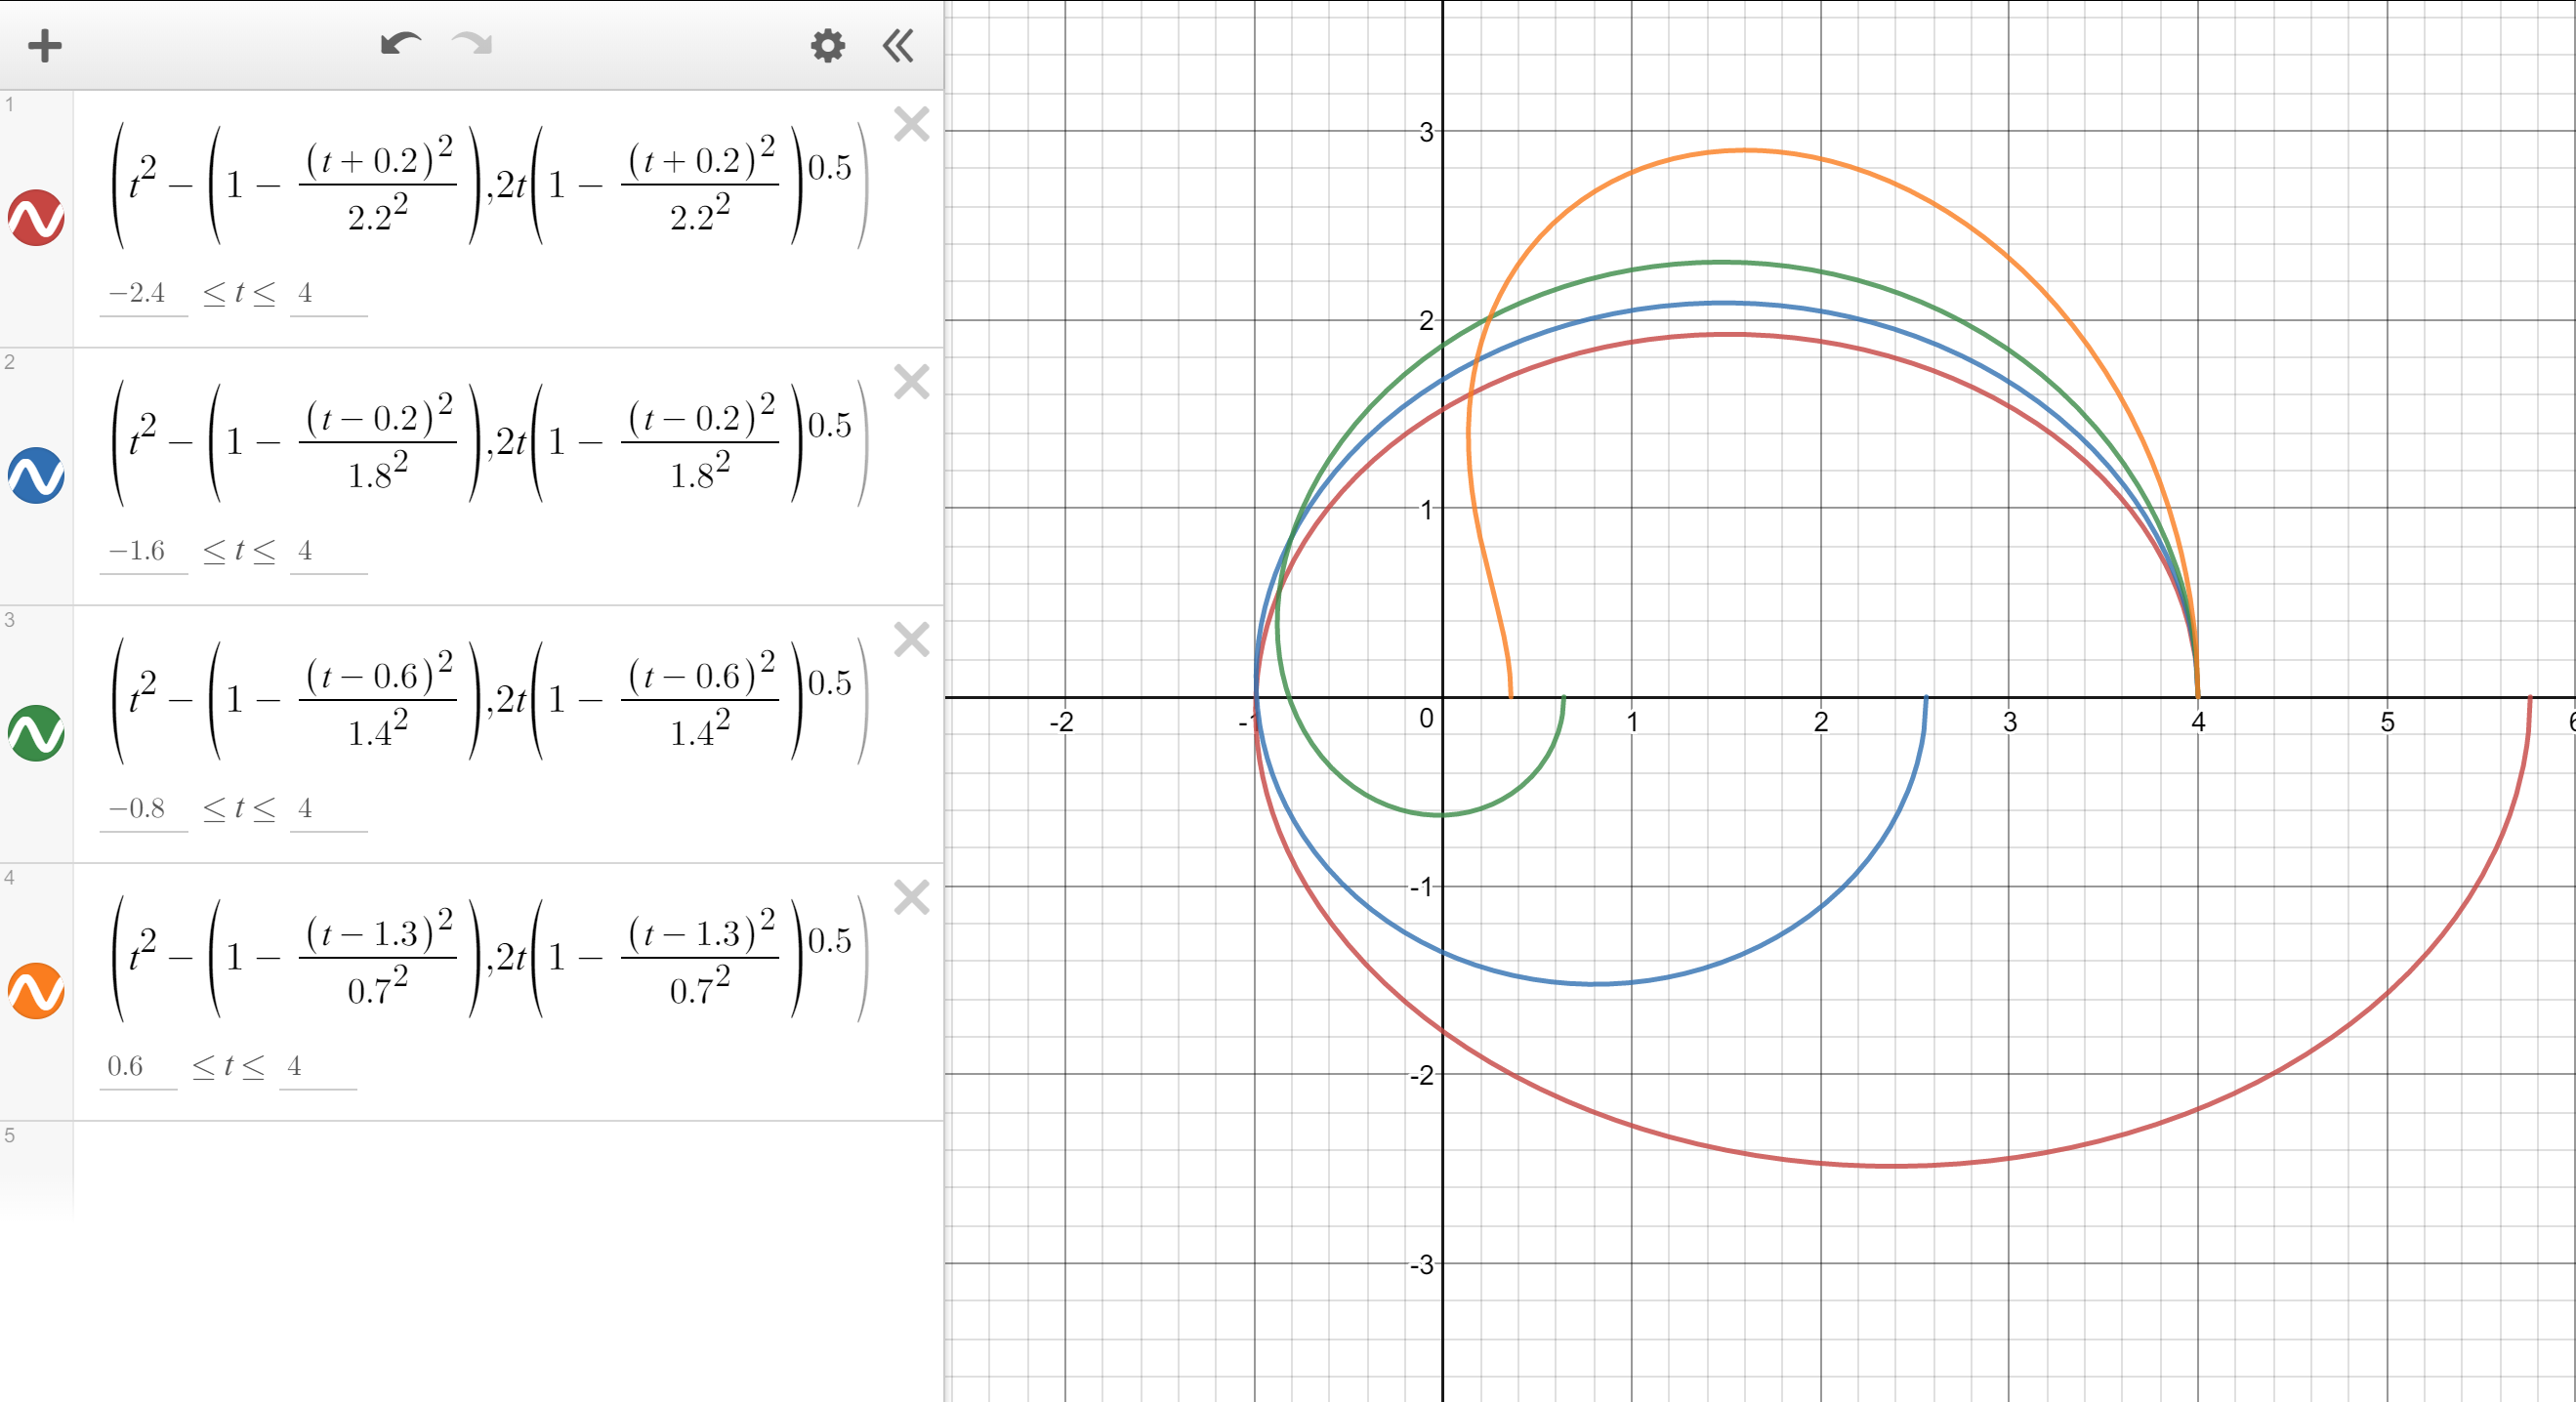
\includegraphics[scale=0.26]{5she2}
    \caption{1-2}
    \end{figure}

\subsection*{2 }
\indent a. we note that $u|u^a,u^b$, also $\varphi$ is continuous, then $\partial D_1 \cap \partial V_2= \varphi(S^1) \simeq S^1$. Deformation contract from regions in $D_1$ and $V_2$ to  $\varphi(S^1)$ in Figure 2. We know that $D_1, V_2, D_1 \cap V_2$ are all path-connected, (here also note by contraction $\pi(V_2)=\pi(D^1\times S^1)=\pi(S^1)=\Z$ ) apply SvK Theorem II, the colimit is $\pi_1(D_1)*_{\pi_1(D_1\cap V_2)}\pi_1(V_2)=1*_{\pi_1(S^1)} \Z =1*_{\Z} \Z $.

Now we proceed to find the relations of generators.  have orientation on $D_1\cap V_2\cong S^1$ as given, name the generator in $\Z$ as $[\gamma]$. Then thus $i_1:\pi_1(D_1\cap V_2) \rightarrow \pi_1(D_1) $ sends generator $[\gamma]\in \Z \textrm{ to } 1 \in 1$; Also we shall notice that we identified $S^1$ in $\C$ , thus we say $u\rightarrow u^{\alpha}$ in virtue rotate $u$ with $a Arg(u)$, w.r.t. real axis. Another map $i_2:\pi_1(D_1\cap V_2) \rightarrow \pi_1(V_2) $ (which is $\pi_1(D_1\cap V_2) \hookrightarrow  \pi_1(S^1\times S^1)=\Z \times \Z \rightarrow \pi_1(V_2)=1 \times \Z$), then this sends $[\gamma]\in \Z \textrm{ to } [1,\Gamma^b] \in \Z$ (Figure $2$).  So eventually $1*_{\pi_1(D_1\cap V_2)}\Z \cong \langle \Gamma ; \Gamma^b=1\rangle$. \\  

b. Apply the theorem in class we know that $\pi_1(V_1)=\pi_1(B^2\times S_1)=\pi_1(B_2)\times \pi_1(S^1)=1\times \Z =\Z$.
$\phi$ is continuous, then $\partial V_1 \cap \partial V_2= \phi(S^1\times S^1) \simeq S^1\times S^1$. Deformation contract from regions in $V_1$ and $V_2$ to  $\varphi(S^1\times S^1)$ in Figure 2. We know that $V_1, V_2, V_1 \cap V_2$ are all path-connected, apply SvK Theorem II, the colimit is $\pi_1(V_1)*_{\pi_1(V_1\cap V_2)}\pi_1(V_2)=\Z*_{\Z\times \Z} \Z$. 

Consider ${i_i}_*:\pi_1(V_1\cap V_2)=\pi_1(S^1\times S^1) \rightarrow \pi_1(V_i)=\pi_1(1\times S^1) $, it kills first component, as contraction. Also notice ${i_i}_*$ is a homomorphism. (These will be used later)  

Now we proceed to find the relations of generators. We have orientation on $V_1\cap V_2\cong S^1{\times} S^1$ as given, name the generator in $\Z \times \Z$ as $[\gamma_1,\gamma_2]$. We identified $\pi_1(V_1)=\pi_1(V_2)\cong \Z$, and (by part a  we shall notice that we identified $S^1$ in $\C$ , thus we say $u\rightarrow u^{\alpha}$ in virtue rotate $u$ with $a Arg(u)$, w.r.t. real axis) along with several other maps: ${i_1},{i_2}$ . We notice, since ${i_1}_*,{i_2}_*$ are (previously) homomorphisms, can thus consider ${i_j}_*([\gamma_1,\gamma_2])={i_j}_*([\gamma_1]){i_j}_*([\gamma_2]) $ and further obtain mapped generators. Then ${i_1}_*([\gamma_1],1)=1$ (by previous), ${i_1}_*(1,[\gamma_2])=\Gamma_1$; ${i_2}_*([\gamma_1],1)=\Gamma_2^b$ (by given map), ${i_2}_*(1,[\gamma_2])=\Gamma_2^d$.

We have $i_1:\pi_1(V_1\cap V_2)  \rightarrow \pi_1(V_1) $ sends generator $[\gamma_1,\gamma_2]\in \Z \times \Z \textrm{ to } \Gamma_1 \in \Z$;  Another map $i_2:\pi_1(V_1\cap V_2) \rightarrow \pi_1(V_2) $ then sends $[\gamma_1,\gamma_2]\in \Z \textrm{ to    } \Gamma_2^{b}\Gamma_2^{d} $ (Figure $2$).  So eventually \\ $\Z*_{\Z\times \Z} \Z \cong \langle \Gamma_1,\Gamma_2; \textrm{   }\Gamma_2^b=1,\Gamma_1\Gamma_2^d=1\rangle$. 


A  diagram is below (Figure 2).
    \begin{figure}[h!]
    \centering
    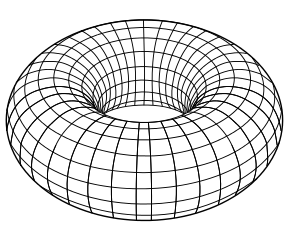
\includegraphics[scale=0.5]{Simple_Torus_svg}
    \caption{2}
    \end{figure}

\end{document}

\frac{\pi}{}